%%%%%%%%%%%%%%%%%%%%%%%%%%%%%%%%%%%%%%%%%%%%%%%%%%%%%%%%
%%%%%%%%%%%%%%%%%%%%%%%%%%%%%%%%%%%%%%%%%%%%%%%%%%%%%%%%
%%%%%%%%%%%%%%%%%%%%%%%%%%%%%%%%%%%%%%%%%%%%%%%%%%%%%%%%
\chapter{Clustering}
\label{chap:cluster}

%%%%%%%%%%%%%%%%%%%%%%%%%%%%%%%%%%%%%%%%%%%%%%%%%%%%%%%%
%%%%%%%%%%%%%%%%%%%%%%%%%%%%%%%%%%%%%%%%%%%%%%%%%%%%%%%%
\section{Evaluating Performance}
\label{cluster:eval}
% TODO

%%%%%%%%%%%%%%%%%%%%%%%%%%%%%%%%%%%%%%%%%%%%%%%%%%%%%%%%
\subsection{Davies-Bouldin Index}
\label{cluster:eval:davies_bouldin}
% TODO

\begin{equation} \label{eq:davies_bouldin}
\text{DB} = \frac{1}{m} \sum_{i=1}^{m} \max_{i \neq j} \left(\frac{\sigma_{i} + \sigma_{j}}{\abs{\mathbf{c}_{i} - \mathbf{c}_{j}}}\right)
\end{equation}

%%%%%%%%%%%%%%%%%%%%%%%%%%%%%%%%%%%%%%%%%%%%%%%%%%%%%%%%
\subsection{Adjusted Rand Index}
\label{cluster:eval:adjusted_rand_index}
% TODO

%%%%%%%%%%%%%%%%%%%%%%%%%%%%%%%%%%%%%%%%%%%%%%%%%%%%%%%%
\subsection{Shannon Index}
\label{cluster:eval:shannon_index}
% TODO

%%%%%%%%%%%%%%%%%%%%%%%%%%%%%%%%%%%%%%%%%%%%%%%%%%%%%%%%
\subsection{Silhouette Coefficient}
\label{cluster:eval:silhouette}
% TODO

%%%%%%%%%%%%%%%%%%%%%%%%%%%%%%%%%%%%%%%%%%%%%%%%%%%%%%%%
%%%%%%%%%%%%%%%%%%%%%%%%%%%%%%%%%%%%%%%%%%%%%%%%%%%%%%%%
\section{\texorpdfstring{$k$}{k}-Means}
\label{cluster:kMean}
% TODO

%%%%%%%%%%%%%%%%%%%%%%%%%%%%%%%%%%%%%%%%%%%%%%%%%%%%%%%%
\subsection{Choosing \texorpdfstring{$k$}{k}: Elbow Method}
\label{cluster:kMean:elbow}
% TODO

%%%%%%%%%%%%%%%%%%%%%%%%%%%%%%%%%%%%%%%%%%%%%%%%%%%%%%%%
\subsection{Metrics}
\label{cluster:kMean:metrics}
% TODO

\subsubsection{Cartesian Radius}
\label{cluster:kMean:metrics:cartesian}
% TODO

% \begin{equation}\label{eq:cartesian}
% \end{equation}

\subsubsection{Cosine Simularity}
\label{cluster:kMean:metrics:cos}
% TODO

% \begin{equation}\label{eq:cos}
% \end{equation}

%%%%%%%%%%%%%%%%%%%%%%%%%%%%%%%%%%%%%%%%%%%%%%%%%%%%%%%%
%%%%%%%%%%%%%%%%%%%%%%%%%%%%%%%%%%%%%%%%%%%%%%%%%%%%%%%%
\section{Expectation Maximization (EM)}
\label{cluster:EM}
% TODO

%%%%%%%%%%%%%%%%%%%%%%%%%%%%%%%%%%%%%%%%%%%%%%%%%%%%%%%%
\subsection{Gaussian Mixture Model (GMM)}
\label{cluster:EM:GMM}
% TODO

%%%%%%%%%%%%%%%%%%%%%%%%%%%%%%%%%%%%%%%%%%%%%%%%%%%%%%%%
%%%%%%%%%%%%%%%%%%%%%%%%%%%%%%%%%%%%%%%%%%%%%%%%%%%%%%%%
\section{Louvain Method}
\label{cluster:louvain}

When working with a graph, \ie network, based dataset
we can use the Louvain\footnote{Named for the location of the author's university in Louvain-la-Neuve, Belgium.} method \cite{louvain}
to detect related clusters, \ie communities,
of nodes by optimizing the graph's modularity\footnote{Today the Louvain method can refer to the greedy optimization algorithm on its own,
with the modularity $Q$ being one possible objective function}.
The modularity $Q$ of a graph $G$ with a given set of clusters $C$
is a measure of the graph's degree of clustering;
being the fraction of edges within the clusters
minus the expected fraction if the edges were randomly distributed.
In short, we can think of $Q$ as a measure of
the density of interior to exterior edges of the clusters.
$Q$ ranges from \num{-0.5} for relatively uncluttered graphs
to \num{1} for fully clustered graphs.
We can compute the modularity $Q$ of $G$ as:

\begin{equation} \label{eq:unsupervised:louvain:modularity}
Q\left(G\right) = \frac{1}{2 W_{G}} \sum_{ij \in G} \bigg(w_{ij} - \gamma \frac{W_{i} W_{j}}{2 W_{G}}\bigg) \delta\left(c_{i},\,c_{j}\right)
\end{equation}

\noindent where\footnote{Note $w_{ij}=1$ for an unweighted graph, and $2 W_{G} = \sum_{ij \in G} w_{ij}$ accounts for double counting edges.}
$w_{ij}$ is the edge weight between nodes $i$ and $j$,
$W_{i}$ is the sum of edge weights of node $i$,
$W_{G}$ is the total edge weight of the graph,
$c_{i} \in C$ is the cluster of node $i$,
and $0 < \gamma$ is a resolution hyperparameter.

The Louvain method constructs $C$ by greedily maximizing $Q$ in an iterative two phase process as shown in \cref{fig:louvain}.
In the first phase, we define each node $n_{i} \in G$ to be its own cluster $c_{i}$.
We then merge each $c_{i}$ with the neighboring $c_{j}$, $0 < w_{ij}$, which maximizes $\Delta Q$.
If $\max\left(\Delta Q\right) = 0$ we leave $c_{i}$ unmerged.
After all clusters have been merged and $Q$ is at a local maximum we enter the second phase.
Here a new graph $G'$ is constructed by making each cluster $c_{i}$ into a node $n'_{i} \in G'$.
The old weights of $G$ are summed to become the new weights $w'_{ij}$,
with intra-cluster weights becoming self-loops $w'_{ii}$ in $G'$.
We return to the first phase and repeat until $Q$ has been maximized.

\begin{figure}
\centering
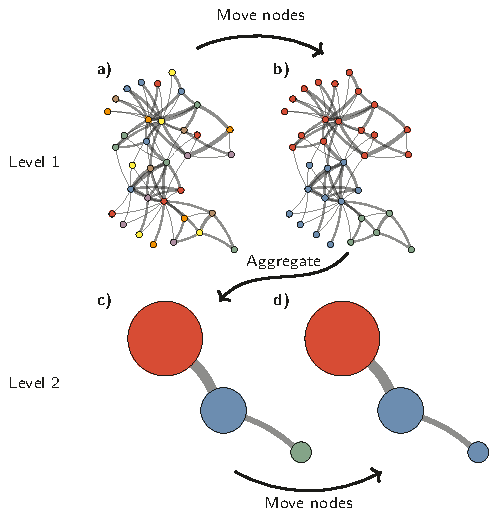
\includegraphics[width=0.5\textwidth]{figures/ml/louvain_algo}
\caption{
Illustration of the two iterative phases of the Louvain method \cite{leiden}.
}
\label{fig:louvain}
\end{figure}

The resolution parameter $\gamma$ controls the number and size of clusters, $\gamma =1$ by default.
The location of $\gamma$ depends on the text and implementation,
but here $1 < \gamma$ ($\gamma < 1$) favors more (fewer) clusters with fewer (more) constituent nodes.
The \texttt{python-louvain}
\href{https://python-louvain.readthedocs.io/en/latest/}{package} \cite{python-louvain}
implements the Louvain method for \texttt{networkx} \cite{networkx}
\href{https://networkx.org/}{based graphs}.
Community detection in large networks is an important problem for social networks and other use cases,
making this an active area of research.
For example, one proposed improvement to the Louvain method is the Leiden algorithm \cite{leiden}.

%%%%%%%%%%%%%%%%%%%%%%%%%%%%%%%%%%%%%%%%%%%%%%%%%%%%%%%%
%%%%%%%%%%%%%%%%%%%%%%%%%%%%%%%%%%%%%%%%%%%%%%%%%%%%%%%%
\section{Correlation Clustering}
\label{cluster:correlation}
% TODO

%%%%%%%%%%%%%%%%%%%%%%%%%%%%%%%%%%%%%%%%%%%%%%%%%%%%%%%%
%%%%%%%%%%%%%%%%%%%%%%%%%%%%%%%%%%%%%%%%%%%%%%%%%%%%%%%%
\section{Affinity Clustering}
\label{cluster:affinity}
% TODO

%%%%%%%%%%%%%%%%%%%%%%%%%%%%%%%%%%%%%%%%%%%%%%%%%%%%%%%%
%%%%%%%%%%%%%%%%%%%%%%%%%%%%%%%%%%%%%%%%%%%%%%%%%%%%%%%%
\section{Support Vector Clustering}
\label{cluster:SVC}
% TODO

